\documentclass[usenames,dvipsnames, 9pt]{beamer}
\usepackage{amsmath,amsfonts,amssymb}
\usepackage{mathtools}
\usepackage{etex} %for Windows
\usepackage[utf8]{inputenc}
\usepackage[english, russian]{babel} 
%\usepackage{microtype}			% Better interword spacing and additional kerning.
\usepackage{ellipsis}			% Adjusted space with \dots between two words.
\usepackage{graphicx}
\usepackage{pstricks}

\usepackage{xcolor}


\usepackage{changepage}

\usepackage{algorithm}
\usepackage{algpseudocode}
%\usepackage[]{algorithm2e}
%\usepackage{algorithmic}

%\usepackage{tcolorbox}






\usepackage{tikz}
\usetikzlibrary{tikzmark,calc}
\usetikzlibrary{positioning, backgrounds}
\usetikzlibrary{arrows, chains, matrix, scopes, patterns, shapes, fit}
\usetikzlibrary{mindmap,trees,shadows}
\usetikzlibrary{decorations.pathreplacing}
\usetikzlibrary{crypto.symbols}

\usepackage{pgfplots}

\pgfmathdeclarefunction{gauss}{2}{%
	\pgfmathparse{1/(#2*sqrt(2*pi))*exp(-((x-#1)^2)/(2*#2^2))}%
}


\tikzset{
	invisible/.style={opacity=0},
	visible on/.style={alt={#1{}{invisible}}},
	alt/.code args={<#1>#2#3}{%
		\alt<#1>{\pgfkeysalso{#2}}{\pgfkeysalso{#3}} % \pgfkeysalso doesn't change the path
	},
}

\newcommand\strikeout[2][]{%
	\begin{tabular}[b]{@{}c@{}} 
		\makebox(0,0)[cb]{{#1}} \\[-0.2\normalbaselineskip]
		\rlap{\color{Orange}\rule[0.5ex]{\widthof{#2}}{1.5pt}}#2
\end{tabular}}

\newcommand\Fontvi{\fontsize{11}{13.2}\selectfont}

\usepackage{listings} % for C++ code

\usepackage{braket}
%\usepackage[braket, qm]{qcircuit}



\usepackage[T1]{fontenc}
%\usepackage[sfdefault,scaled=.85]{FiraSans}
%\usepackage{newtxsf}
%\usepackage[nomap]{FiraMono}





\usefonttheme[onlymath]{serif}
\renewcommand\sfdefault{cmbr}

\renewcommand{\bfdefault}{sb}

\definecolor{CharCoalDark}{RGB}{13, 16, 19}
\definecolor{Orange}{RGB}{255, 165,0}
\definecolor{DarkOrange}{RGB}{255, 165,0}
\definecolor{LightSalmon}{RGB}{255, 160, 122}
\definecolor{LeafGreen}{RGB}{34, 139,  34}
\definecolor{Coral}{RGB}{255, 127, 80}
\definecolor{DarkTurquoise}{RGB}{0, 206, 209}

%\newtheorem{defRus}{Определение}
%\newtheorem{thmRus}{Теорема}
%s\newtheorem{corRus}{Следствие}


\setbeamercolor{background canvas}{bg=CharCoalDark}

\setbeamerfont{title}{series=\bfseries}
\setbeamercolor{title}{fg=Orange}
\setbeamercolor{section in toc}{fg=white}
\setbeamercolor{frametitle}{fg=Orange}
\setbeamercolor{normal text}{fg=white}
%\setbeamercolor{normal text}{fontsize=12pt}
\setbeamercolor{itemize item}{fg=Orange}
\setbeamercolor{enumerate item}{fg=Orange}
\setbeamercolor{enumerate item item}{fg=Orange}
\setbeamercolor{itemize item item}{fg=Orange}
\setbeamercolor{enumerate item}{fg=Orange}
\setbeamercolor{block title}{bg=DarkOrange,fg=white}
\setbeamerfont{block title}{series=\bfseries}

\setbeamertemplate{itemize item}[circle]
\setbeamertemplate{eumerate subitem}{\color{Orange}[$\checkmark$]}
\setbeamertemplate{itemize subitem}{\color{Orange}\Large$\textbullet$}
\setbeamertemplate{itemize subitem}{\color{Orange} \tiny $\blacksquare$}

% footnote without a marker
\newcommand\blfootnote[1]{%
	\begingroup
	\renewcommand\footnoterule{}
	\renewcommand\thefootnote{}\footnote{#1}%
	\addtocounter{footnote}{-1}%
	\endgroup
}

\newcommand*{\Scale}[2][4]{\scalebox{#1}{\ensuremath{#2}}}%

\newcommand\Item[1][]{%
	\ifx\relax#1\relax  \item \else \item[#1] \fi
	\abovedisplayskip=0pt\abovedisplayshortskip=0pt~\vspace*{-\baselineskip}}

\pgfdeclareradialshading{ring}{\pgfpoint{0cm}{0cm}}%
{rgb(0cm)=(1,1,1);
	rgb(0.7cm)=(1,1,1);
	rgb(0.719cm)=(1,1,1);
	rgb(0.72cm)=(0.975,0,0);
	rgb(0.9cm)=(1,1,1)}

\usepackage[absolute,overlay]{textpos} %to clip to a corner
\newcommand\FrameText[1]{%
	\begin{textblock*}{\paperwidth}(\textwidth-35pt, 10 pt)
		\raggedright #1\hspace{.5em}
\end{textblock*}}

\makeatletter
\let\save@measuring@true\measuring@true
\def\measuring@true{%
	\save@measuring@true
	\def\beamer@sortzero##1{\beamer@ifnextcharospec{\beamer@sortzeroread{##1}}{}}%
	\def\beamer@sortzeroread##1<##2>{}%
	\def\beamer@finalnospec{}%
}
\makeatother

\AtBeginSection[]
{
	\begin{frame}<beamer>
		\frametitle{Outline}
		\tableofcontents[currentsection]
	\end{frame}
}


%\institute{ENS Lyon}
\author{Elena Kirshanova \\ [10pt]
}
\titlegraphic{
	
	%\includegraphics[width=2.5cm]{erc_logo_gray}\hspace*{2.5cm}~%
	%\includegraphics[width=4.0cm]{ens_logo_gray}
}
\title{\Huge Modes of Operations.}

\date{ Course ``Information and Network Security'' \\ 	
	Lecture 4 \\ \today }


\setbeamertemplate{navigation symbols}{} %removes navigation

% proper highlightling of a code-snippet
\lstset{language=C++,
	keywordstyle=\color{magenta},
	stringstyle=\color{Goldenrod},
	commentstyle=\color{gray},
	breaklines=false,
	%morecomment=[l][\color{magenta}]{\#}
}

%\setlength{\parskip}{8pt}
% ==================================================================
% Definitions for this paper
% ==================================================================
\mathchardef\hyphen="2D

\usepackage{multirow}
\usepackage{multicol} % For multiple coloumn environments
%\usepackage{stmaryrd} % For set brackets
% \setlength{\columnsep}{15pt} % Defining the coloumn seperation
% \setlength{\columnseprule}{1pt} % Place a line between coloumns
% \newcommand{\tab}{\hspace*{2em}}

%subscripts

\newcommand*\SmallTextScript[2]{{\mathchoice{\displaystyle #2}
		{\textstyle #2}%dito
		{\scalebox{#1}{\ensuremath{\scriptstyle #2}}}%
		{\scalebox{#1}{\ensuremath{\scriptscriptstyle #2}}}%
}}


% ADVERSARIES AND SUCH
\newcommand*{\poly}{\ensuremath{\mathrm{poly}}}
\newcommand*{\eps}{\ensuremath{\varepsilon}}
\newcommand*{\alg}{\ensuremath{\mathcal{A}}}

% GROUPS/DISTRIBUTIONS/SETS/LISTS
\newcommand{\N}{{{\mathbb N}}}
\newcommand{\Z}{{{\mathbb Z}}}
\newcommand*{\IZ}{\ensuremath{\mathbb{Z}}}
\newcommand*{\IN}{\ensuremath{\mathbb{N}}}
\newcommand*{\IQ}{\ensuremath{\mathbb{Q}}}
\newcommand{\R}{{{\mathbb R}}}
\newcommand*{\IR}{{{\mathbb R}}}
\newcommand{\Zp}{\Z_p} % Integers modulo p
\newcommand{\Zq}{\Z_qs} % Integers modulo q
\newcommand{\Zn}{\ints_N} % Integers modulo N
\newcommand{\F}{\ensuremath{\mathbb{F}}}
\newcommand{\CC}{\ensuremath{\mathbb{C}}}

\newcommand{\ord}{\ensuremath{\mathrm{ord}}}

\newcommand{\GF}{\ensuremath{\mathbb{F}_2}}
\newcommand{\GFn}{\ensuremath{\mathbb{F}^n_2}}

%%% ALGORITHMS/PROCEDURES %%%
\newcommand{\Dec}{\textsf{Dec}}
\newcommand{\Enc}{\textsf{Enc}}
\newcommand{\KeyGen}{\textsf{KeyGen}}
\newcommand{\Gen}{\textsf{Gen}}
\newcommand{\MAC}{\textsf{MAC}}
\newcommand{\sk}{\textsf{sk}}
\newcommand{\pk}{\textsf{pk}}
\newcommand{\mesS}{\ensuremath{\mathcal{M}}}
\newcommand{\keyS}{\ensuremath{\mathcal{K}}}
\newcommand{\cipS}{\ensuremath{\mathcal{C}}}
\newcommand{\tagS}{\ensuremath{\mathcal{T}}}
\newcommand{\nonceS}{\ensuremath{\mathcal{N}}}
\newcommand{\mactag}{\textsf{tag}}
\newcommand{\Hash}{\ensuremath{\mathcal{H}}}
\newcommand{\EID}{\ensuremath{\mathtt{EphID}}}

\newcommand{\rem}{\ensuremath{\mathrm{rem}}}

\newcommand{\adv}{\ensuremath{\mathcal{A}}}

\newcommand{\LWE}{\mathsf{LWE}}
\newcommand{\DCP}{\mathsf{DCP}}
\newcommand{\EDCP}{\mathsf{EDCP}}
\newcommand{\UEDCP}{\mathsf{U \text{-} EDCP}}
\newcommand{\GEDCP}{\mathsf{G \text{-} EDCP}}



%% Landau and proba
\newcommand{\bigO}{\mathcal{O}}
\newcommand*{\OLandau}{\bigO}
\newcommand*{\WLandau}{\Omega}
\newcommand*{\xOLandau}{\widetilde{\OLandau}}
\newcommand*{\xWLandau}{\widetilde{\WLandau}}
\newcommand*{\TLandau}{\Theta}
\newcommand*{\xTLandau}{\widetilde{\TLandau}}
\newcommand{\smallo}{o} %technically, an omicron
\newcommand{\wLandau}{\omega}
\newcommand{\negl}{\mathrm{negl}}
\newcommand*\PROB\Pr 
\DeclareMathOperator*{\EXPECT}{\mathbb{E}}
\DeclareMathOperator*{\VARIANCE}{\mathbb{V}}
\DeclareMathOperator*{\LOGBIAS}{\mathbb{LB}}

\newcommand{\supp}{\ensuremath{\mathsf{sup}}}
\newcommand{\Distr}{\ensuremath{\mathcal{D}}}

% Lattices

% \newcommand{\coset}{\Lambda} % Lambda Lattice
% \newcommand{\cosetPerp}{\Lambda^{\bot}} % Lambda_Perp Lattice
% \newcommand{\gadget}{\textbf{G}} %Gaget matrix
% \newcommand{\mes}{\textbf{m}} %message vector
% \newcommand{\AMat}{\textbf{A}} %A matrices
% \newcommand{\BMat}{\textbf{B}} %B matrices
% \newcommand{\RMat}{\textbf{R}} %R matrices
% \newcommand{\HMat}{\textbf{H}} %H matrices
% \newcommand{\XMat}{\textbf{X}} %H matrices
% \newcommand{\mbar}{\bar{m}} %mBar dimension
% % \newcommand{\gauss}{\mathcal{D}} % gaussian distribution
% \newcommand{\Id}{\textbf{I}} % Identity matrix
% \newcommand{\er}{\textbf{e}} % gaussian distr. vectors
% % \newcommand{\cipher}{\textit{c}} % ciphertext
% \newcommand{\Olwe}{\mathcal{O}_{\textsf{LWE}}} %LWE oracle
% \newcommand{\OSample}{\mathcal{O}_{Sample}} %LWE oracle
% \newcommand{\SigmaB}{\boldsymbol{\Sigma}} %semi-deifinite matrix Sigma%
% % \newcommand{\mods}{\text{ mod}}


%Vectors and Matrices

\newcommand{\AMat}{\mathbf{A}} %A matrices
\newcommand{\BMat}{\mathbf{B}} %B matrices
\newcommand{\DMat}{\mathbf{D}} %Diagonal


\newcommand{\HMat}{\ensuremath{\mathbf{H}}}
\newcommand{\QMat}{\ensuremath{\mathbf{Q}}}
\newcommand{\Id}{\ensuremath{\mathbf{I}}}
\newcommand{\ZeroM}{\textbf{0}} % Zero matrix

\newcommand{\avec}{\ensuremath{\mathbf{a}}}
\newcommand{\bvec}{\ensuremath{\mathbf{b}}}
\newcommand{\cvec}{\ensuremath{\mathbf{c}}}
\newcommand{\evec}{\ensuremath{\mathbf{e}}}
\newcommand{\rvec}{\ensuremath{\mathbf{r}}}
\newcommand{\svec}{\ensuremath{\mathbf{s}}}
\newcommand{\tvec}{\ensuremath{\mathbf{t}}}
\newcommand{\vvec}{\ensuremath{\mathbf{v}}}
\newcommand{\zvec}{\ensuremath{\mathbf{z}}}
\newcommand{\xvec}{\ensuremath{\mathbf{x}}}
\newcommand{\yvec}{\ensuremath{\mathbf{y}}}
\newcommand{\uvec}{\ensuremath{\mathbf{u}}}
\newcommand{\zerovec}{\ensuremath{\mathbf{0}}}

\newcommand{\nth}{^{\mathrm{th}}}
\newcommand{\nd}{^{\mathrm{nd}}}

\newcommand{\RepMMT}{\ensuremath{\mathcal{R}_{\protect\SmallTextScript{0.70}{\texttt{MMT}}}}}
\newcommand{\RepBJMM}{\ensuremath{\mathcal{R}_{\protect\SmallTextScript{0.70}{\texttt{BJMM}}}}}
\newcommand{\XOR}{\ensuremath{\mathtt{3XOR}}}


% % % % % \newcommand{\mb}[1]{\mathbf{#1}} % does not compile otherwise
%%% Removed by Gotti; this is just asking to screw up with packages that (properly) define \mb (mathbold)

% \newcommand{\bL}{\|\bvec_1\|} % b1 length that appears way too often
% \newcommand{\dL}{\|\dvec_1\|} % b1 length that appears way too oftend

%Norms and Scalar products

\newcommand*\abs[1]{\left\lvert#1\right\rvert}
\newcommand*\norm[1]{\left\lVert#1\right\rVert}
\newcommand*\normalabs[1]{\lvert#1\rvert} 
\newcommand*\normalnorm[1]{\lVert#1\rVert}
\newcommand*\bignorm[1]{\bigl\lVert#1\bigr\rVert}
\newcommand*\bigabs[1]{\bigl\lvert#1\bigr\rvert}
\newcommand*\Bigabs[1]{\Bigl\lvert#1\Bigr\rvert}
\newcommand*{\ScProd}[2]{\ensuremath{\langle#1\mathbin{,}#2\rangle}} %Scalar Product
% \newcommand*{\ScProd}[2]{\ensuremath{\langle#1 \:{,}\:#2\rangle}} %Scalar Product
\newcommand*{\bigScProd}[2]{\ensuremath{\bigl\langle#1\mathbin{,}#2\bigr\rangle}} %Scalar Product
\newcommand*{\BigScProd}[2]{\ensuremath{\Bigl\langle#1\mathbin{,}#2\Bigr\rangle}} %Scalar Product
\newcommand{\dist}{\ensuremath{\text{dist}}}


%Some other math operators

\DeclareMathOperator{\Span}{Span} %span of vectors
\DeclareMathOperator{\vol}{\mathrm{vol}} %volume
\DeclareMathOperator{\LW}{LambertW} %Lambert W function
\DeclareMathOperator{\SD}{SD}
\DeclareMathOperator{\gradient}{grad}
\DeclareMathOperator{\TRACE}{Tr}
\newcommand*{\dDR}{\mathrm{d}} %de-Rham-Differential (the d in dx, dy, dz and so on)


%Lists
\renewcommand{\L}{\ensuremath{\mathcal{L}}}

\renewcommand{\P}{\ensuremath{\mathcal{P}}}

\newcommand*{\Lout}{\ensuremath{\L_{\mkern-0.5mu\protect\SmallTextScript{0.85}{\textup{out}}}}}
\newcommand*{\Sout}{\ensuremath{S_{\mkern-0.5mu\protect\SmallTextScript{0.85}{\textup{out}}}}}
\newcommand{\wt}{\ensuremath{\mathit{wt}}}


\newcommand*{\softO}{\widetilde{\bigO}}

\newcommand{\const}{\mathsf{c}} 


\newcommand{\transpose}{\mkern0.7mu^{\mathsf{ t}}}

%proper overline reduced by 1.5mu
\newcommand{\overbar}[1]{\mkern 1.5mu\overline{\mkern-1.5mu#1\mkern-1.5mu}\mkern 1.5mu}

\DeclareMathOperator{\erf}{erf} %error function
\DeclareMathOperator{\erfc}{erfc} %complementary error function
\newcommand{\Er}{\ensuremath{\mathrm{Er}}} %complementary error function


% LATTICES

\newcommand{\Lat}{\ensuremath{\mathcal{L}}}
\newcommand*{\Sphere}[1]{\ensuremath{\mathsf{S}^{#1}}}
%\DeclareMathOperator{\Conf}{Conf}
\newcommand{\Conf}{\mathcal{C}}

%Thick line for table
\setlength{\doublerulesep}{0pt}
\newcommand{\thickline}{\hline\hline\hline}


%circled text
\newcommand*\circled[1]{\tikz[baseline=(char.base)]{
    \node[shape=circle,draw,inner sep=0.3 pt] (char) {\scriptsize #1};}}


%Fix Algorithmicx package
\def\NoNumber#1{{\def\alglinenumber##1{}\State #1}\addtocounter{ALG@line}{-1}}

%For comments
\newcommand{\GColor}{ForestGreen}  %Damiens' color
\newcommand{\EColor}{MidnightBlue} %Elena's color

\newcommand*{\E}[1]{{\color{\EColor} #1} } 
\newcommand*{\G}[1]{{\color{\GColor} #1} } 

%Proper limit with the subscript underneath
% \newcommand{\Lim}[1]{\raisebox{0.5ex}{\scalebox{0.8}{$\displaystyle \lim_{#1}\;$}}}


%TIKZ dense dotted pattern

\pgfdeclarepatternformonly{my dots}{\pgfqpoint{-1pt}{-1pt}}{\pgfqpoint{2.0pt}{2.0pt}}{\pgfqpoint{2pt}{2pt}}%
{
	\pgfpathcircle{\pgfqpoint{0pt}{0pt}}{.35pt}
	\pgfpathcircle{\pgfqpoint{1pt}{1pt}}{.35pt}
	\pgfusepath{fill}
}


\tikzset{
	master/.style={
		execute at end picture={
			\coordinate (lower right) at (current bounding box.south east);
			\coordinate (upper left) at (current bounding box.north west);
		}
	},
	slave/.style={
		execute at end picture={
			\pgfresetboundingbox
			\path  (lower right)rectangle (upper left) ;
		}
	}
} %all defs
\begin{document}
	
\begin{frame}
	\titlepage
\end{frame}


\begin{frame}{Recap: Block ciphers}
\LARGE 

\begin{itemize}
	%\itemsep 1em
	\item Most popular primitive for symmetric encryption
	\item Core element: a {\color{Orange} public} function $f$
	\[
		f (x, k) \quad x \in \mesS, \, k \in \keyS \text{ such that }
	\]
	$f$ is  {\color{Orange} efficient} and {\color{Orange} secure$^\star$}
	\item we iterate $f$ over several rounds
\end{itemize}
\begin{figure}
	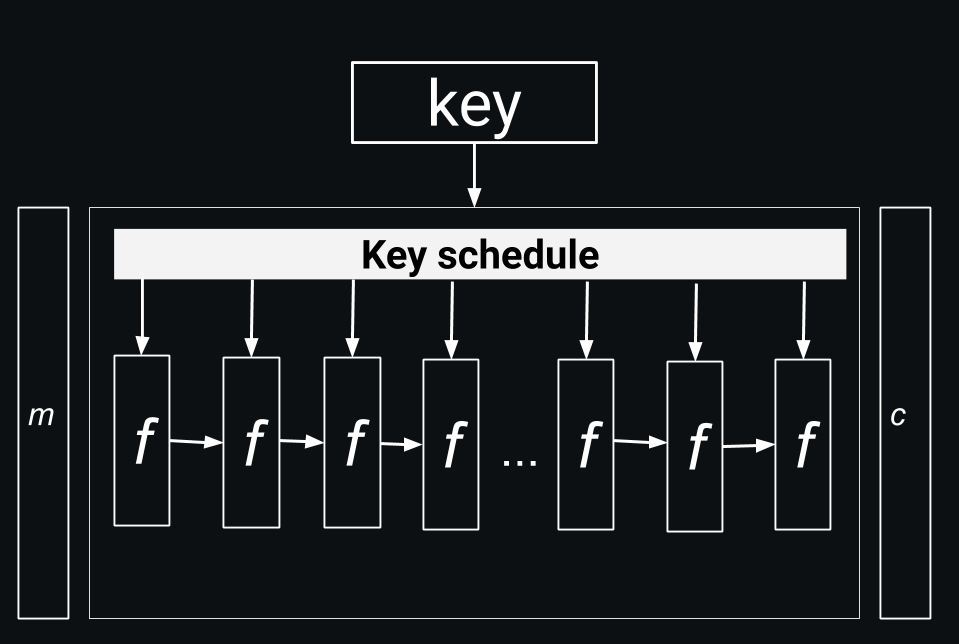
\includegraphics[width=0.65\textwidth]{BlockCipherGeneral}
\end{figure}

	\vfill  {\normalsize $\star$ a secure block cipher is non-trivial to define }

\end{frame}

\begin{frame}{Recap: Block ciphers}
\Large
There are two main design principals of rounds
\vspace{10pt}
%\LARGE
\begin{columns}
	\centering
	\begin{column}{0.45\textwidth}
		{\color{Orange}Feistel cipher}
		%\vspace{20pt}
		\centering
		\tikzmark{start}
		\includegraphics[width=0.6\textheight]{Feistel2}
		\tikzmark{end} 
	\end{column}

\begin{column}{0.55\textwidth}
	{\color{Orange}Substitution Permutation Network }
	\centering
	\tikzmark{start}
	\includegraphics[width=0.65\textheight]{SPN}
	\tikzmark{end} 
\end{column}
\end{columns}

\end{frame}

\begin{frame}{Recap: Block ciphers}

\begin{itemize}
	\itemsep 2em
	\LARGE
	\item Feistel cipher \\
	 -- Usually requires more rounds to achieve `good mixing' \\[5pt]
	-- Easy to invert: iterate in reverse  \\[5pt]
	\Large
	Examples: DES, ГОСТ 28147-89
	\LARGE
	\item Substitution-Permutation Network (SPN). \\ Подстановочно-перестановочная сеть  \\[5pt]
	-- Used in modern protocols  \\[5pt]
	-- Inversion is non-trivial \\[5pt]
	\Large
	Examples: AES, ГОСТ 34.12-2018
	
\end{itemize}
\end{frame}

\begin{frame}
	\Huge
	\centering
	{\color{Orange}How to use a block cipher correctly?} \\[10pt]
	
	Modes of operation.
	
\end{frame}

\begin{frame}{Electronic Block Code (EBC)}

\Large
Let $m = (m_1, m_2, m_3, ...)$ \\
A naive way to use a block cipher $B$
\begin{figure}
			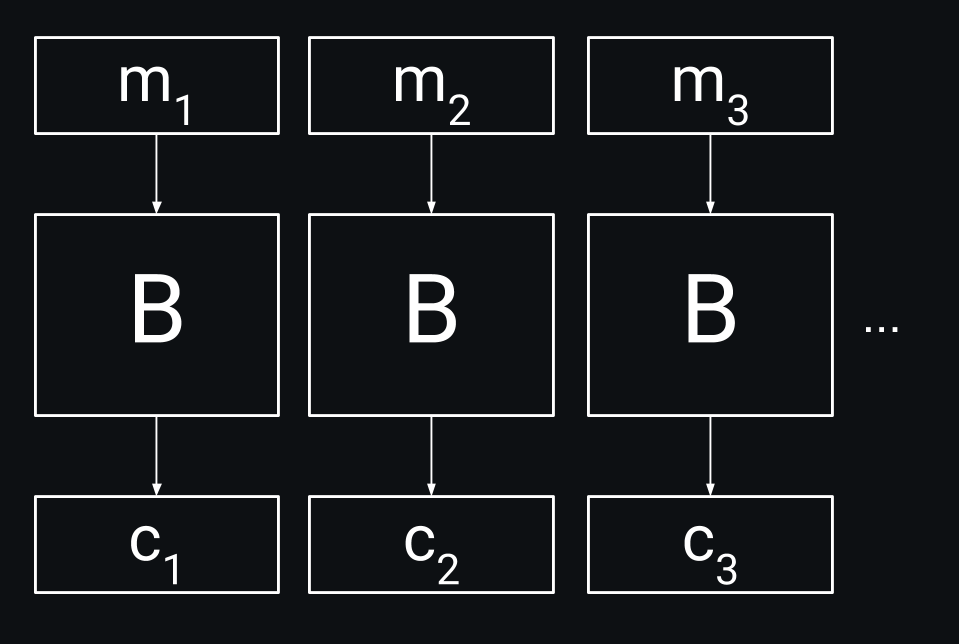
\includegraphics[width=0.9\textwidth]{EBC}
	\end{figure}
\LARGE
This is {\color{Orange} INSECURE!} \quad
If $m_1 = m_2$ then $c_1 = c_2$

\end{frame}

\begin{frame}{Insecurity of EBC}
\centering
\Huge If $m_1 = m_2$ then $c_1 = c_2$ \\[20pt]
\large
\begin{figure}
	\includegraphics[width=0.3\textwidth]{Tux} \quad 
	\includegraphics[width=0.3\textwidth]{Tux_ecb} \quad 
	\includegraphics[width=0.3\textwidth]{Tux_secure}
\end{figure}

\vfill
\small
{\color{gray} \textsuperscript{\textcopyright} Wikipedia} 
\end{frame}

\begin{frame}{Cipher Block Chain (CBC)}
\Large
{\color{Orange} IV} -- Initial Vector -- a random bit string

\begin{figure}
	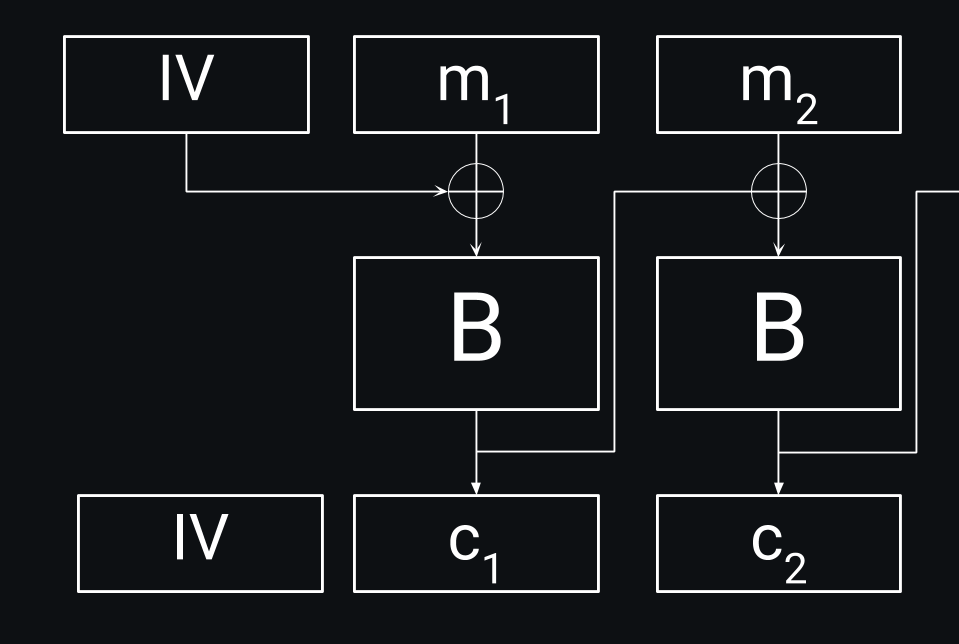
\includegraphics[width=0.95\textwidth]{CBC}
\end{figure}
IV is a part of a ciphertext, i.e., publicly known
\end{frame}

\begin{frame}{Security of Cipher Block Chain (CBC)}
\Large
\begin{itemize}
\item The IV must be {\color{Orange} unpredictable} (if an attacker predicts IV, encryption with CBC is not secure).\\ 
Known vulnerability in TLS 1.1 (ciphertext of a message was used as IV for the next message). 
\pause 
\item{\color{Orange} IV must be updated}  \\

\end{itemize}
\end{frame}

\begin{frame}{Security of Cipher Block Chain (CBC)}
	Assume we encrypt under the same IV a very long message $m=(m_1, \ldots, m_t)$ for $t> 2^{n/2}$ where $n$ is the block length ($n=128$ for AES, GOST'15)
	\vspace{-10pt}
	\begin{figure}
		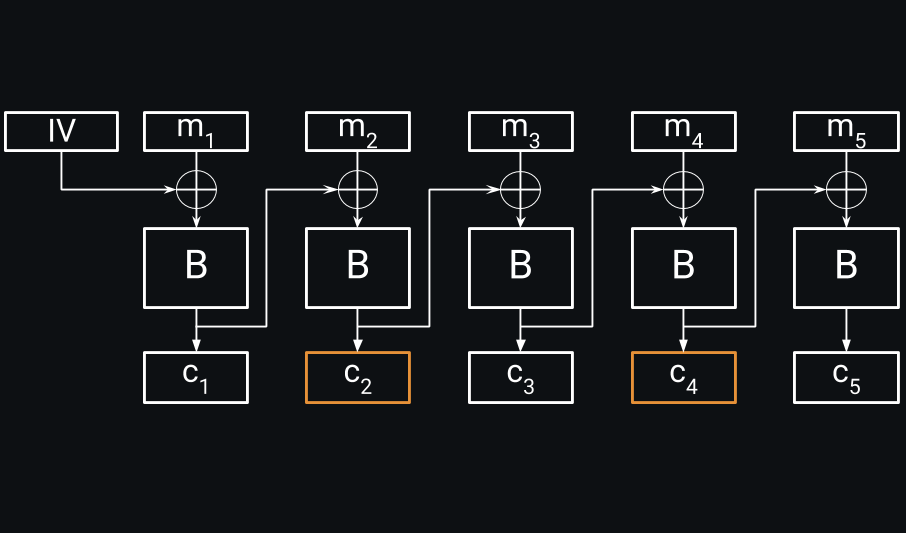
\includegraphics[width=1\textwidth]{CBC_1}
	\end{figure}
\vspace{-40pt}
{\color{Orange}Birthday paradox:} after seeing ~$2^{n/2}$ cipher-text blocks $c_i$'s, with high probability two of them will be equal, e.g.,  $c_2 == c_4$ Therefore,
\Large
\[
	c_1 \oplus m_2 == c_3 \oplus m_4
\]
Statistical attacks can be applied.
\end{frame}

\begin{frame}{Birthday Paradox}
\Large
	Q: Is it more likely that some two people in the room  of 30 people share the same birthday or that no two people in the room share the same birthday?\\
	\pause
	Simple calculations$^\star$ reveal that the 2nd event happens with probability
	\[
		\left(1 - \frac{1}{365}\right)  \left(1 - \frac{2}{365}\right) \left(1 - \frac{3}{365}\right) \cdot \ldots \cdot \left(1 - \frac{29}{365}\right)  \approx 0.294
	\]
	Hence, with probability $>70\%$ there are two people sharing the same birth date.
	\vfill  {\normalsize $\star$ see any introductory textbook  on probability theory}
\end{frame}

\begin{frame}{Birthday Paradox}
\Large
In general, if there are $m$ people and $N$ possible birthdays, the probability that all $m$ have different birthdays is
\[
	\prod_{i=1}^{m-1} \left(  1  -\frac{i}{N} \right) \approx e^{-m^2/2N}
\]

Hence, for $m = \sqrt{2N \ln 2}$, the probability that all $m$ people have different birthdays is $1/2$.  This probability decreases rapidly when $m$ grows. \\[10pt]

\pause
In block ciphers on block length $n$, we have $2^{n}$ possible ciphers.\\
After $m = \bigO(2^{n/2})$ different cipher blocks $c_i$'s, two of them are equal with constant probability.\\
\pause
For CBC mode: $c_i == c_j$ for $m=(m_1, \ldots, m_t)$, $t \approx 2^{n/2}$:
\Large
\[
c_{i-1} \oplus m_{i} == c_{j-1} \oplus m_{j}
\]

\end{frame}


\begin{frame}{Padding for CBC}
\Large
The CBC mode requires padding
\begin{figure}
	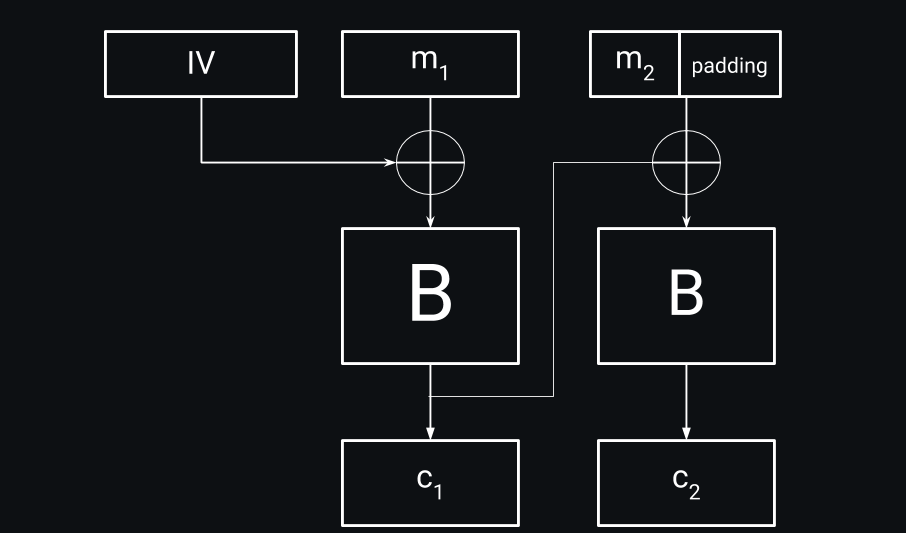
\includegraphics[width=0.85\textwidth]{CBC_Padding}
\end{figure}
Usually $n$-byte padding is consists of $n$ copies of $n$: i.e., $5$ bytes padding is $5|5|5|5|5$. If $m$ is less than the block-length, we add a dummy block.
\end{frame}

\begin{frame}{Counter Mode (CTR)}
\Large
Modern way to use block ciphers \\
Now IV - initial value of a counter: it is incremented for each new message block. Only the initial value of IV is transmitted.
\begin{figure}
	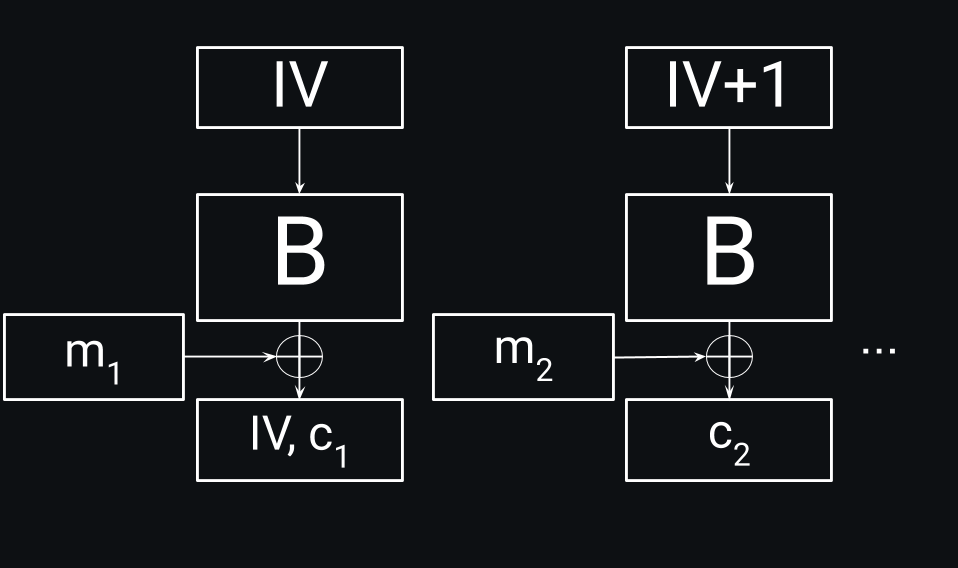
\includegraphics[width=0.95\textwidth]{CTR}
\end{figure}
\vspace{-20pt}
This is a way to turn a block cipher into a stream cipher \\

\end{frame}

\begin{frame}{Example of a Shape of IV}
	\begin{figure}
		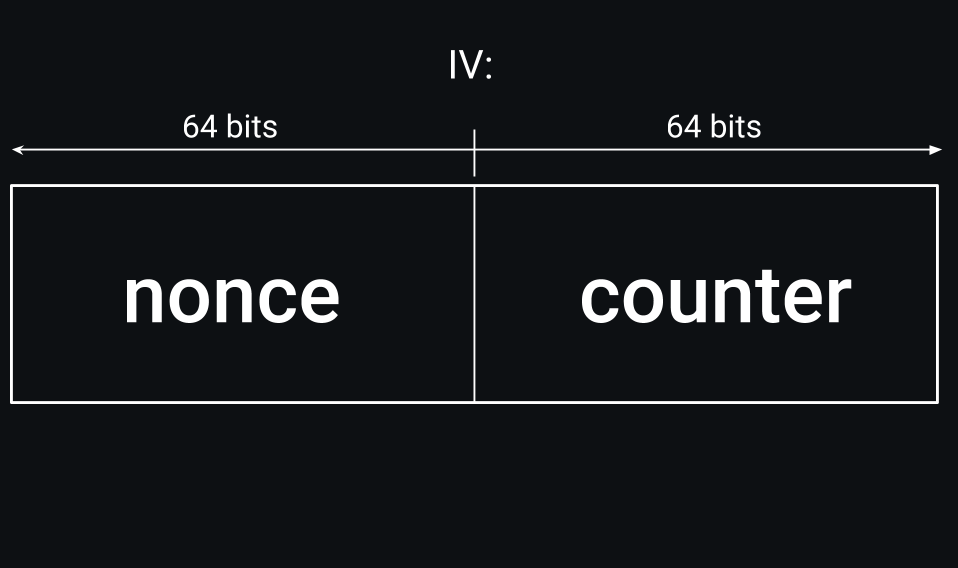
\includegraphics[width=0.95\textwidth]{ShapeOfIV}
	\end{figure}
\vspace*{-40pt}
\large
\begin{itemize}
\item Nonce should be unpredictable (a 64-bit output of a PRG) and should never repeat for the same key $k$\\
\item Counter increments for every message block
\item Do to need to transmit the counter in protocols that guarantee in-order delivery (e.g., https)
\item Can use one nonce for at most $2^{64}$ message blocks, i.e., refresh the nonce after $2^{64}$ encryptions

\end{itemize}
\end{frame}


\begin{frame}{Counter Mode (CTR)}
%\vspace{-40pt}
\begin{figure}
	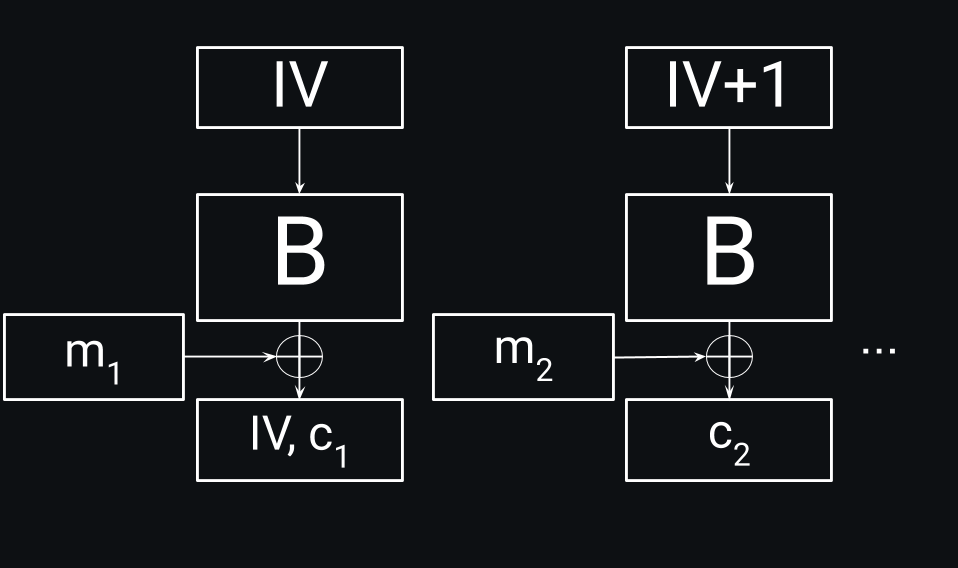
\includegraphics[width=0.55\textwidth]{CTR}
		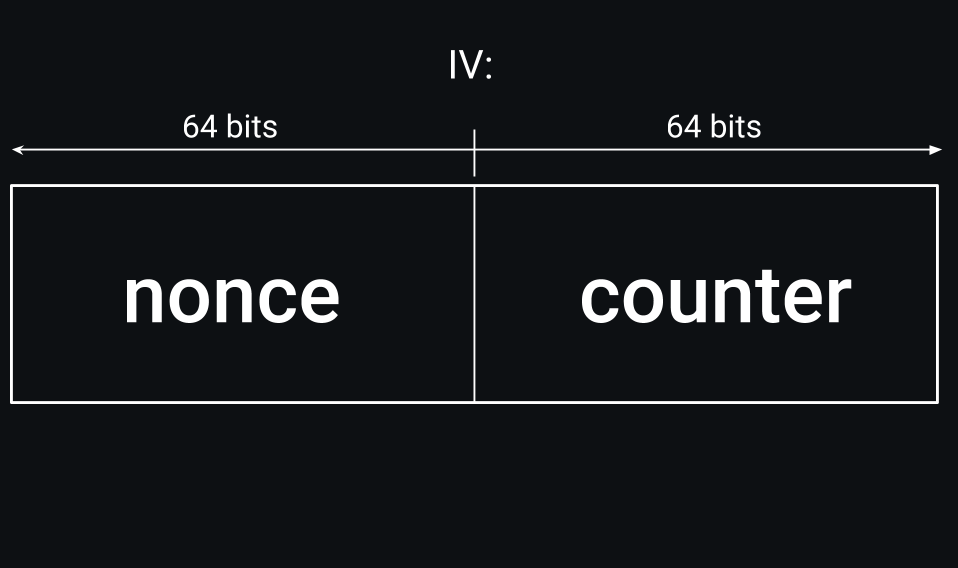
\includegraphics[width=0.45\textwidth]{ShapeOfIV}
\end{figure}
%\vspace{-20pt}
\Large
\begin{itemize}
	\item Nonce is known to both encryptor and decryptor 
	\item Advantage: Simple decryption routine
	\item Advantage: Can be parallelized (unlike CBC)
	\item Advantage: No need to use padding
\end{itemize}

\end{frame}


\begin{frame}{Take-away}

\LARGE

\begin{enumerate}
	\itemsep 2em
	\item {\color{Orange} DO NOT} use the EBC mode 
	\item  The CBC mode, used in old TLS, {\color{Orange} is inferior to} the CTR mode
	\item Use the CTR mode in your constructions
	
\end{enumerate}
\end{frame}

\begin{frame}{Programming assignment}

\Large

{\color{Orange} Task:} encrypt a text file with AES  \\[10pt]

Details and useful links are in the instructions file\\[10pt]

Send your questions and finished assignments to \\[10pt]

\centering

\url{elenakirshanova@gmail.com}



\end{frame}


\begin{frame}{Feedback}
	Please leave your anonymous feedback at \\[10pt]
	\url{https://docs.google.com/forms/d/e/1FAIpQLSfVLhzxzbuxhAawoESWaCL50146ktDwVRXMLK5FeXzFTzuGTA/viewform?usp=sf_link}
	
	
\end{frame}


\end{document}